\section{Multiple network representation learning}
\label{sec:ch6:multinet}

In this section, we're going to learn a number of strategies that are useful from when we have multiple networks. When we have multiple networks, there are a variety of questions that we might want to ask. In this section, we'll focus on a few of these questions, and provide structured ways to learn representations of these networks that allow us to address our downstream questions. We'd recommend that you glance back at the $COSIE_{n, M}\left(V, \{R_m\}_{m = 1}^M\right)$ random networks in Section \ref{sec:ch5:multi}, as these will be critical for understanding many of the techniques that we cover in this section.

We'll use a running example of brain networks, which we describe in Remark \ref{box:ch6:multinet:ex}.

\begin{floatingbox}[h]\caption{Alien and human brain networks}
\label{box:ch6:multinet:ex}
Let's imagine that you're a brain network, and you've been given the unique task of learning about a group of $4$ human-like alien life forms that were recently discovered. When studying their brains (in a non-invasive way), you make the remarkable discovery that aliens and humans have brain areas that do similar things across species. These $n=100$ brain areas will be the nodes of your network.

For both aliens and humans, there are two hemispheres (communities) in the brain. However, you make a somewhat startling discovery in that while human brains tend to have a homophilic structure (with more connections between nodes in the same hemisphere of the brain), alien brains tend to have a disassortative structure (with more connections between nodes in the opposite hemisphere of the brain).

For this reason, you want to be able to obtain suitable representations of your networks that you can use downstream to learn about the differences between human and alien brain networks.
\end{floatingbox}

Let's generate our working examples:

\begin{lstlisting}[style=python]
from graspologic.simulations import sbm
import numpy as np

n = 100  # the number of nodes
M = 8  # the total number of networks
# human brains have homophilic block structure
Bhum = np.array([[0.2, 0.02], [0.02, 0.2]])
# alien brains have a disassortative block structure
Balien = np.array([[0.02, 0.2], [0.2, 0.02]])

# generate 4 human and alien brain networks
A_humans = [sbm([n // 2, n // 2], Bhum) for i in range(M // 2)]
A_aliens = [sbm([n // 2, n // 2], Balien) for i in range(M // 2)]
# concatenate list of human and alien networks
As = A_humans + A_aliens

# 1 = left hemisphere, 2 = right hemisphere for node communities
zs = [1 for i in range(n // 2)] + [2 for i in range(n // 2)]
labels = ["L" for i in range(n // 2)] + ["R" for i in range(n // 2)]
\end{lstlisting}

The collection \texttt{As} is a list of adjacency matrices, where the first $4$ entries correspond to the human brains, and the second $4$ entries correspond to the alien brains. \texttt{zs} corresponds to community labels for the nodes of the networks, where \texttt{1} is a place-holder for ``Left hemisphere'', and \texttt{2} is a placeholder for ``Right hemisphere''. We also added a second list of community labels, \texttt{labels}, which correspond to the true names. You might find having dummy place-holders for discrete community labels (such as \texttt{zs}) to be handy when you want to do things like run one-hot encodings, and you might find having more informative node labels (such as \texttt{labels}) handy for when you want to visualize, plot, and learn from your networks.

\begin{figure}[h]
    \centering
    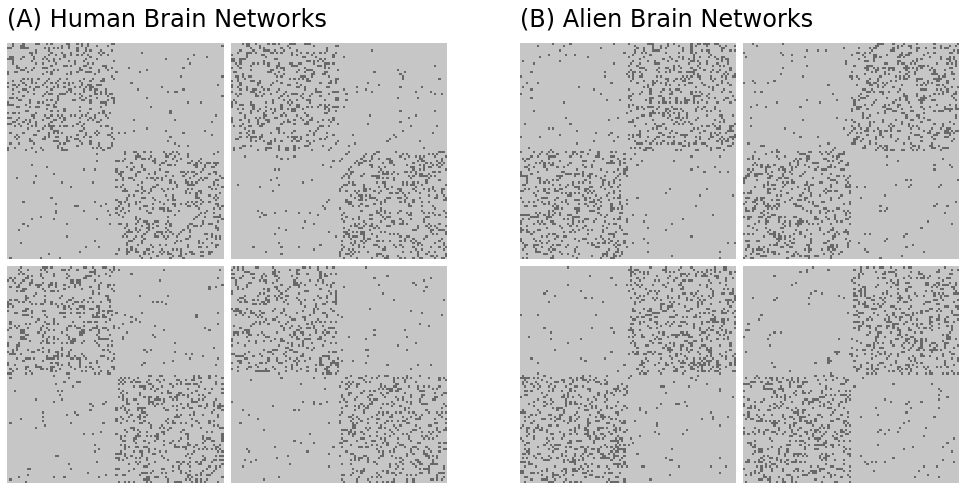
\includegraphics[width=\linewidth]{representations/ch6/Images/multi_ex.png}
    \caption[Alien/Human brain network example]{\textbf{(A)} the human brain networks, and \textbf{(B)} the alien brain networks.}
    \label{fig:ch6:multinet:ex}
\end{figure}
The human and alien brain networks are plotted (nodes are ordered by the node hemisphere, the ``community'') in Figure \ref{fig:ch6:multinet:ex}. Notice that whereas the human brain networks tend to have more connections within the same hemisphere (the on-diagonal blocks), the alien brain networks tend to have more connections between the two hemispheres (the off-diagonal blocks). 

Remember, our goal is to identify whether humans and aliens have similar or different structure to their nodes. We're going to try to to embed our brain networks into some lower-dimensional space. Once the nodes are in a lower dimensional space, we can use standard downstream techniques to learn latent structure from the network.

\subsection{Embedding networks through averaging}

The first place that we might start is to average our networks together, and then embed the result with spectral embedding. It turns out that, if we can safely assume that all of the networks in a collection are similar, in the sense that there is no particular reason that one network should be distinct from another, this is actually the right case. Formally, analyzing embeddings of the average tends to be appropriate when the networks have the same distribution.

As we'll see, based on what we know already, using a naive average and embedding the result is fairly inappropriate for the data. Let's see what happens when we average the networks:

\begin{lstlisting}[style=python]
# compute the global average across all networks
global_mean_network = np.array(networks).mean(axis=0)
\end{lstlisting}

\begin{figure}[h]
    \centering
    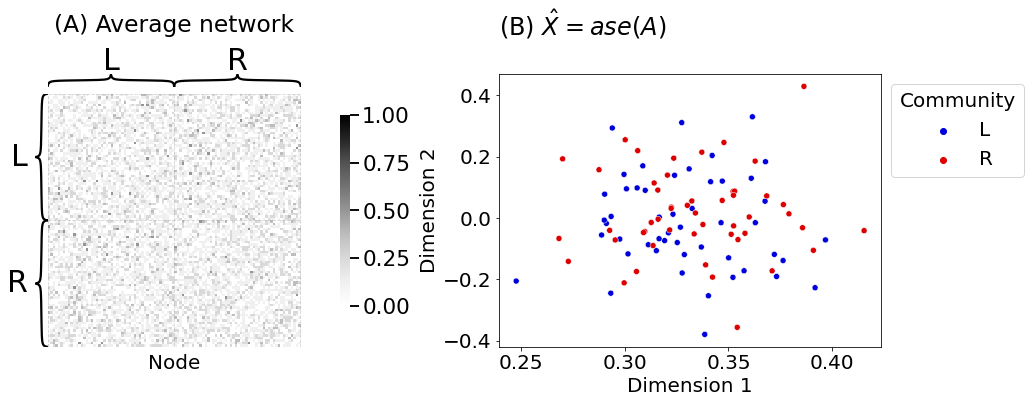
\includegraphics[width=\linewidth]{representations/ch6/Images/multinet_avg.png}
    \caption[Average embedding]{\textbf{(A)} the average network produced by averaging the adjacency matrices for humans and aliens together, \textbf{(B)} the latent positions of the average networks.}
    \label{fig:ch6:multinet:avg}
\end{figure}

We visualize this network as a heatmap in Figure \ref{fig:ch6:multinet:avg}(A). Not that the salient topological structures that we identified in Figure \ref{fig:ch6:multinet:ex} have been decimated, in the sense that they are not visually prominent anymore. This is because our analysis of Figure \ref{fig:ch6:multinet:ex} suggested that the networks had a different underlying block matrix (humans appeared to have a ``homophilic'' structure, and aliens appeared to have a ``dissassortative'' structure). The degree of decimation of structure (visually) is a function of the specific network samples you obtain, as well as the disparity between the underlying random networks.

Next, we embed the result using \texttt{ase}, with a target dimensionality of $2$ since the networks have two communities:

\begin{lstlisting}[style=python]
from graspologic.embed import AdjacencySpectralEmbed as ase
Xhat = ase(n_components=2).fit_transform(global_mean_network)
\end{lstlisting}

We plot the resulting latent position estimates in Figure \ref{fig:ch6:multinet:avg}(B). One thing that should jump out immediately is that, as we might have expected, this approach has severe drawbacks. The decimation of latent structure (visually, in the heatmap) was further reflected in the decimation of structure in the downstream spectral embeddings.

\subsubsection{Conditional averaging and then embedding}

From our initial visualizations in Figure \ref{fig:ch6:multinet:ex}, it might have been easy to predict why the averaging procedure might fail: the networks from our visualizations in \ref{fig:ch6:multinet:ex} had prominent ``opposing'' structures, in that all of the humans showed a homophilic structure, but all of the aliens showed a disassortative structure. As we explored above, when we took a naive average and embedded the result, we decimated structure between the two hemispheres. For this reason, a more principled approach that we might think up would be to average only networks that appear somewhat homogeneous (in terms of the underlying probability matrices).

In this case, we could visually look at the network heatmaps in Figure \ref{fig:ch6:multinet:avg} and immediately conclude that all of the human networks might have a similar block matrix, and all of the alien networks might also have a similar block matrix. Since the probability matrices for $SBM_n(\vec z, B)$ random networks are a function of the community assignments of nodes $\vec z$ (which is the same across the groups of networks) and the block matrix $B$, as we learned in Section \ref{sec:ch5:ier:sbm_pmtx}, we might be able to visually conclude that the human networks are somewhat homogeneous and the alien networks are somewhat homogeneous.

Therefore, it might feel appropriate to \textit{conditionally average}, where we compute averages looking only within a particular group. In this situation, that would entail computing an average adjacency matrix for the human networks, an average adjacency matrix for the alien networks, and then embedding each separately. 

Let's see how this works out for us:

\begin{lstlisting}[style=python]
hum_mean = np.array(A_humans).mean(axis=0)
alien_mean = np.array(A_aliens).mean(axis=0)
\end{lstlisting}
\begin{figure}[h]
    \centering
    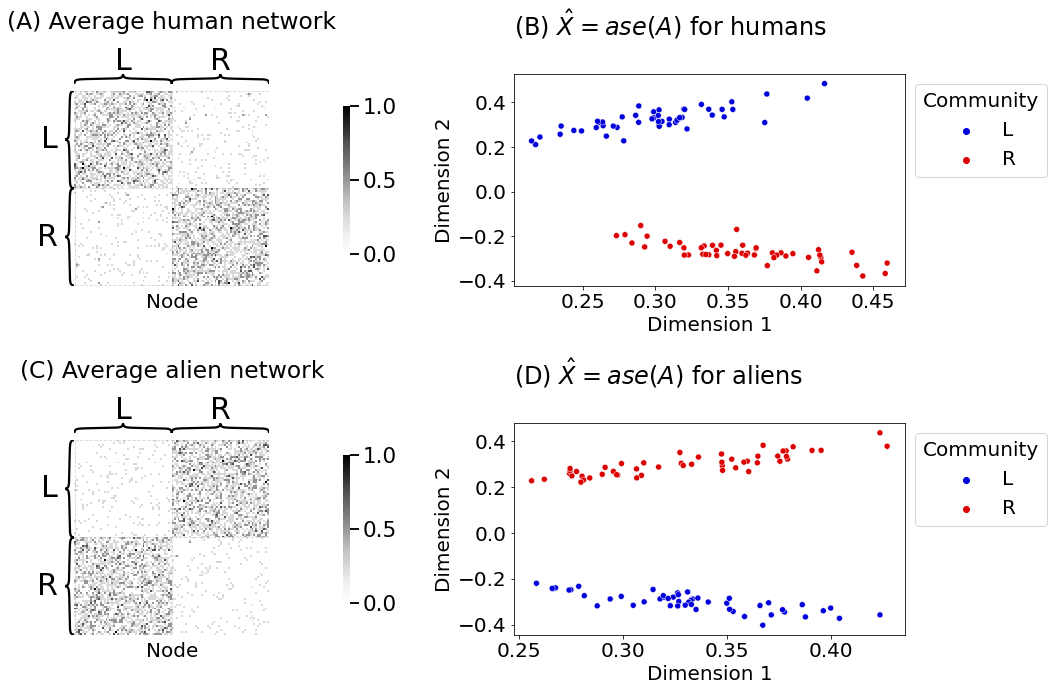
\includegraphics[width=\linewidth]{representations/ch6/Images/cond_avg.png}
    \caption[conditional average embeddings]{\textbf{(A)} the average human adjacency matrix, \textbf{(B)} the spectral embedding of the average human adjacency matrix, \textbf{(C)} the average alien adjacency matrix, \textbf{(D)} the spectral embedding of the average alien adjacency matrix.}
    \label{fig:ch6:multinet:cond_avg}
\end{figure}
We plot the conditional averages in Figure \ref{fig:ch6:multinet:cond_avg}(A) and \ref{fig:ch6:multinet:cond_avg}(C). Note that averaging conditionally has not decimated our known structure to the adjacency matrices.

Next, we embed the conditional averages, again using \texttt{ase}:

\begin{lstlisting}[style=python]
Xhat_hum = ase(n_components=2).fit_transform(hum_mean)
Xhat_alien = ase(n_components=2).fit_transform(alien_mean)
\end{lstlisting}

The latent position estimates for the conditional averages is shown in Figure \ref{fig:ch6:multinet:cond_avg}(B) and \ref{fig:ch6:multinet:cond_avg}(D). When we look at the latent position estimates, it appears that community structure has been preserved, which means that we have not decimated the latent structure that we want to investigate further downstream. This is good news for us, however we have another problem. A reasonable way we might want to approach determining whether human and alien brain networks differ would be to compare the latent position estimates, right? Unfortunately, this is not that easy to do, due to the problem we mentioned in Section \ref{sec:ch6:spectral:nonidentifiable}, the non-identifiability problem. Particularly, the estimates that we produced for humans and aliens, \texttt{Xhat\_hum} and \texttt{Xhat\_alien}, might not be rotated in the same orientation. 

\subsubsection{What other problems does taking averages suffer from?}

There are a variety of reasons why averaging, even when we conditionally average human and alien brain networks separately, are unideal. When we average the network unconditionally, we can decimate latent structure, like we learned right above. Even when we average the networks conditionally, if all human brain networks and all alien brain networks come from the same distribution, we still encounter problems. The networks end up, potentially disasterously, not being properly oriented in comparable latent spaces, due to the non-identifiability problem. This means that while we could learn (with conditional averaging) about the humans and alien brain networks separately, we could not learn about them together. Our analysis would be restricted to each group of networks individually.

Finally, and potentially most catastrophically, is the big assumption that we made to average the networks conditionally: that all human brain networks, or separately all alien brain networks, come from the same distribution. This assumption, when viewed through a statistical lens, makes little sense: individual to individual, or more generally network to network, it seems rather unreasonable to believe that numerous samples would come from exactly same distribution. In fact, in many cases where it would be desirable to analyze multiple networks, this is the {opposite} of the reason we might analyze multiple networks in the first place. 

Additionally, in light of the concern that we first brought up in Section \ref{sec:ch5:sbm:modularity}, the shared structure (or disparate structure) that exists between our networks might not be immediately obvious to we. If the human and alien brain networks were simply had their nodes not pre-arranged in community order, that humans had a homophilic structure and aliens had a disassortative structure would not have been visually perceptible. 

While we might anticipate there is shared structure between groups of networks that are in the same categories, more often than not, it's going to make sense to choose techniques that are not limited in their level of reasonability to cases where the assumptions of shared structure are imposed (e.g., by averaging). This holds true with the example we gave back in multiple network modelling in \Section \ref{sec:ch5:multi} (where we discussed social networks from Facebook, Twitter, and Linkedin), it holds true in many cases where you look at brain networks like here, and it's going to make sense in many other domains.

In any case where we have reason to believe that each network comes from a unique distribution, we are going to want a way to reflect that in our algorithm. Let's see how we might approach the problem with these limitations of averaging in mind. 

\subsection{Different types of multiple network representation learning}

Let's take a moment to explore some of the possible general approaches we could take in multiple-network representation learning. At some point we need to combine the many individual representations of our networks into one, and there are at least three possible places where we could do this: combining the networks together, combining the networks separately, and combining the embeddings. Each of these eventually results in a latent position representation for our networks. It's important to note that in all of these approaches, we are simply learning representations for our groups of networks. 

All types of multiple-network representation learning strategies that we describe in this section entail first constructing a joint matrix. A \textit{joint matrix} is a matrix which is derived from multiple networks, and summarizes them in such a way that it facilitates downstream analysis. The specific way that the joint matrix is determined from the data depends on the specific multiple-netework representation learning technique.

\subsubsection{Combining the networks together}

With this approach, we start with a set of networks, and then the joint matrix will represent the adjacency matrix of a new network (that summarizes information about all of the other networks that went into it). We then embed and analyze the joint matrix and its embedding directly. What we did before, averaging the human and alien networks, was an example of combining our networks -- we  averaged all of our adjacency matrices, and then we embedded the result. 

This tends to be effective when you want to study a property which is common across all of the networks, and you believe network-to-network differences that do not relate to the property of interest to be effectively noise. Unfortunately, it suffers from many of the issues we just mentioned. This approach is summarized in Figure \ref{fig:ch6:multinet:comb}.

\begin{figure}[h]
    \centering
    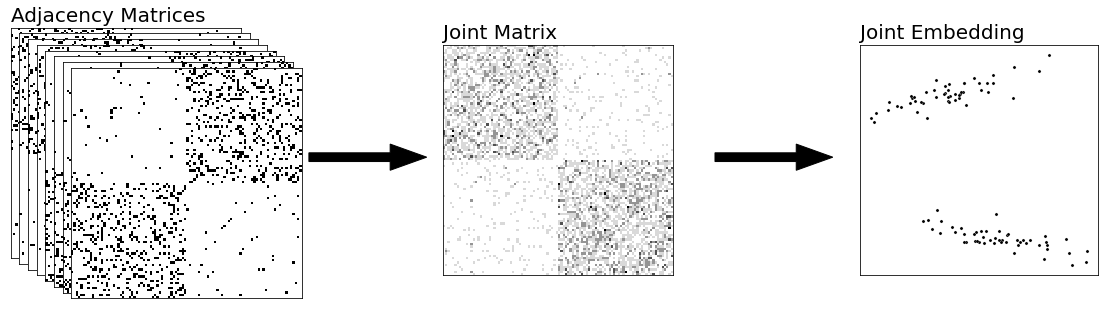
\includegraphics[width=\linewidth]{representations/ch6/Images/joint_comb.png}
    \caption[Combining networks together]{The process of combining your networks to acquire a joint matrix, and then embedding the result to obtain a multiple network representation.}
    \label{fig:ch6:multinet:comb}
\end{figure}

\subsubsection{Combining the embeddings}

The next approach to multiple-network representation learning that we will learn about is combining the embeddings themselves into the joint matrix. With this approach, we first obtain representations from each network, either with adjacency spectral embedding or with some other single-network representation learning strategy. Next, these embeddings are combined into a joint matrix, and then we learn from this joint matrix using sequential approaches (such as additional embeddings of the joint matrix). Multiple adjacency spectral embedding (\texttt{mase}), which we will learn about soon, is an example of this approach. This approach is summarized in Figure \ref{fig:ch6:multinet:comb_emb}.

\begin{figure}[h]
    \centering
    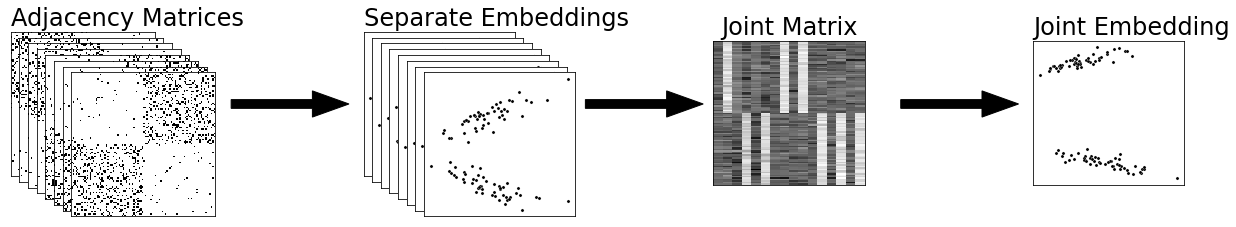
\includegraphics[width=\linewidth]{representations/ch6/Images/comb_emb.png}
    \caption[Combining embeddings together]{The process of embedding your networks to obtain separate representations, combining these individual representations to obtain a joint matrix, and then obtaining a representation of the joint matrix to obtain a multiple network represenatation.}
    \label{fig:ch6:multinet:comb_emb}
\end{figure}


\subsubsection{Combining networks separately}

The above approach is effective when our networks have shared structure, where the final embedding describes shared structures across the nodes of the networks, and we obtain other descriptive features about the joint embedding that describe particularities about the individual networks as they relate to this shared structure. The joint embedding that we obtain tends to summarize information across the nodes, as we will learn soon. 

However, there are situations in which we might want to keep our embeddings separate, with the exception of wanting them to co-exist in a related latent space, meaning the embeddings aren't rotations of each other. This addresses the problem that we noticed in Section \ref{sec:ch6:spectral:nonidentifiable}. When we approach multiple-network representation learning in this manner, we can directly compare the embeddings of the separate networks. An example of combining the networks separately is the Omnibus embedding (OMNI), and is illustrated in Figure \ref{fig:ch6:multinet:comb_sep}.

\begin{figure}[h]
    \centering
    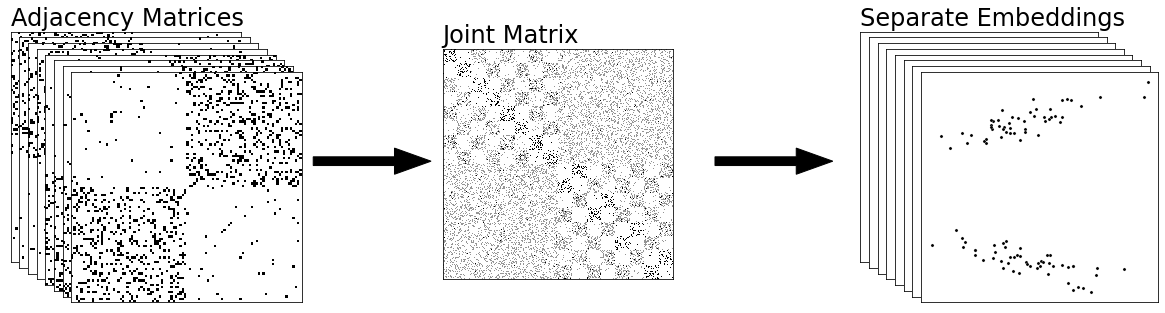
\includegraphics[width=\linewidth]{representations/ch6/Images/comb_sep.png}
    \caption[Combining networks separately]{The process of combining your networks to acquire a joint matrix, and then embedding the result to obtain a multiple network representation.}
    \label{fig:ch6:multinet:comb_sep}
\end{figure}

For the rest of this section, we'll explore the strengths and weaknesses of different techniques which use these latter two approaches. 


\subsection{Multiple Adjacency Spectral Embedding}

Multiple Adjacency Spectral Embedding, or \texttt{mase} is a technique which combines embeddings by concatennating and re-embedding the separate latent positions into a single space. The advantage of \texttt{mase} is we don't actually need each network to be generated from the same distribution - we only need the nodes of the different networks to be aligned and have similar ``meaning'' across the networks. What this means is that node $1$ in network $1$ has the same literal interpretation as node $1$ in networks $2$ through $M$, and so on for all $n$ nodes of the network. In your brain network, for instance, node one is the first region, node two is the second region, ... and this property applies to all of the nodes in the network and across all networks in your collection.

\texttt{mase} is probably the easiest to understand if you know how adjacency spectral embeddings work. We have some number of networks, and (like we said above) their nodes are aligned. The goal of \texttt{mase} is to embed the networks into a shared space with shared latent dimensions. 

\texttt{mase} is based on the common subspace independent-edge (COSIE) model that you learned about in Section \ref{sec:ch5:multi:cosie}. If you recall, with the COSIE model, you learned that across your networks, there might be some underlying homogeneity: in your brain networks, for instance, there might be communities that are shared across all of the networks. Simultaneously, these networks are distinct for one reason or another in terms of the underlying probability matrix: for instance, a pair of humans might have different probabilities for particular edges being connected or disconnected, or a pair of individuals one of whom is human and the other is alien might have different patterns to their probability matrices all together. In this sense, the COSIE model allowed you to capture both the homogeneity and heterogeneity across different networks simultaneously.

Let's go back to your group of human and alien brains and try using \texttt{mase} to embed them rather than averaging. Then, we will dive deeper into what goes on under the hood. 

\begin{lstlisting}[style=python]
from graspologic.embed import MultipleASE as mase

# Use mase to embed everything
mase = mase(n_components=2)
# fit_transform on the human and alien networks simultaneously
# + combines the two lists
latents_mase = mase.fit_transform(networks)
\end{lstlisting}

\subsubsection{How does \texttt{mase} work?}

\paragraph*{Embedding your networks}

The first step in the \texttt{mase} algorithm is to spectrally embed each network. This step is discussed in the preceding sections for \texttt{ase} in Section \ref{sec:ch6:ase} and \texttt{lse} in Section \ref{sec:ch6:lse}. 

When you know ahead of time how many dimensions that you want, you would perform your ASE with the desired number of dimensions here. It is a good rule of thumb to over-embed than it is to under-embed dimensionality wise; that is, if we embed into too many dimensions, we might have more challenges downstream when we try to learn from the networks, but if we embed into too few dimensions, we risk discarding latent structure (and will therefore have no hope of finding it downstream). In general for this first step of \texttt{mase}, a good number of embedding dimensions tends to be $\log_2(n)$. When $n$ is $100$ as in your example, this comes to about $7$:

\begin{lstlisting}[style=python]
from graspologic.embed import AdjacencySpectralEmbed as ase

dhat = int(np.ceil(np.log2(n)))
# spectrally embed each network into ceil(log2(n)) dimensions with ASE
joint_matrix = [ase(n_components=dhat).fit_transform(network) for network in As]
\end{lstlisting}

We plot the spectral embeddings of a human and an alien (showing only the first two dimensions) in Figure \ref{fig:ch6:multinet:mase:ase}. Notice that the separate embeddings individually preserve the community structure across both humans and aliens. Figure \ref{fig:ch6:multinet:mase:ase_joint}(A) shows the embeddings across all networks as heatmaps.

\begin{figure}[h]
    \centering
    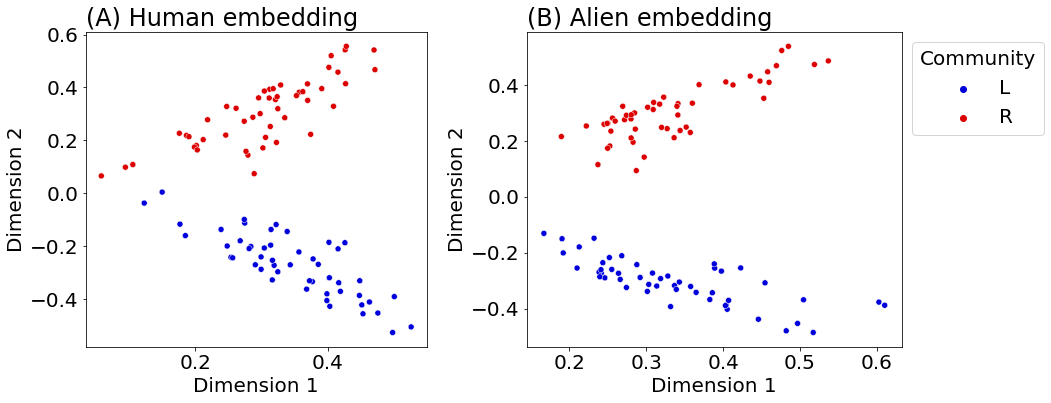
\includegraphics[width=0.8\linewidth]{representations/ch6/Images/mase_ase.png}
    \caption[\texttt{mase} \texttt{ase} step]{\textbf{(A)} the spectral embedding for a human network, and \textbf{(B)} the spectral embedding for an alien network.}
    \label{fig:ch6:multinet:mase:ase}
\end{figure}

It is important to note that these embeddings do not live in the same latent space just yet; that is, they may be oriented differently, and the embeddings are not directly comparable.

\paragraph*{Calculating a shared latent space}

Now comes the interesting part. Our goal is to find some way to take each of these individual embeddings and combine them. We want to find a reasonable way of doing this.

To do this, what we'll effectively do is take each of our individual network embeddings, and concatenate them horizontally. Because the rows of these matrices are all aligned - meaning, row 1 corresponds to node 1 for all four matrices - you can actually think of each node as having (in this case) $Md$ latent dimensions: there are $d$ latent dimensions for each of your $M$ networks. In this case, since $\hat d = 7$ and $M = 8$, this means that each node has $7 \times 8 = 56$ latent dimensions associated with it ($7$ per network).

You don't actually need separate matrices to express this idea: the natural thing to do would be to just concatenate all of the matrices horizontally into a single $n \times Md$ matrix, where $n$ is the number of nodes (the rows of the resulting matrix), and $Md$ is the number of latent dimensions associated with each node (the columns of the resulting matrix). This matrix is called the joint matrix, since it is a composition of information from the $M$ total networks. We can concatenate the adjacency matrices to construct the joint matrix using numpy:

\begin{lstlisting}[style=python]
# Concatenate your embeddings horizontally into a single n x Md matrix
joint_matrix = np.hstack(joint_matrix)
\end{lstlisting}

This matrix is plotted in Figure \ref{fig:ch6:multinet:mase:ase_joint}(B), and is known as the \textit{joint matrix} for \texttt{mase}.

\begin{figure}[h]
    \centering
    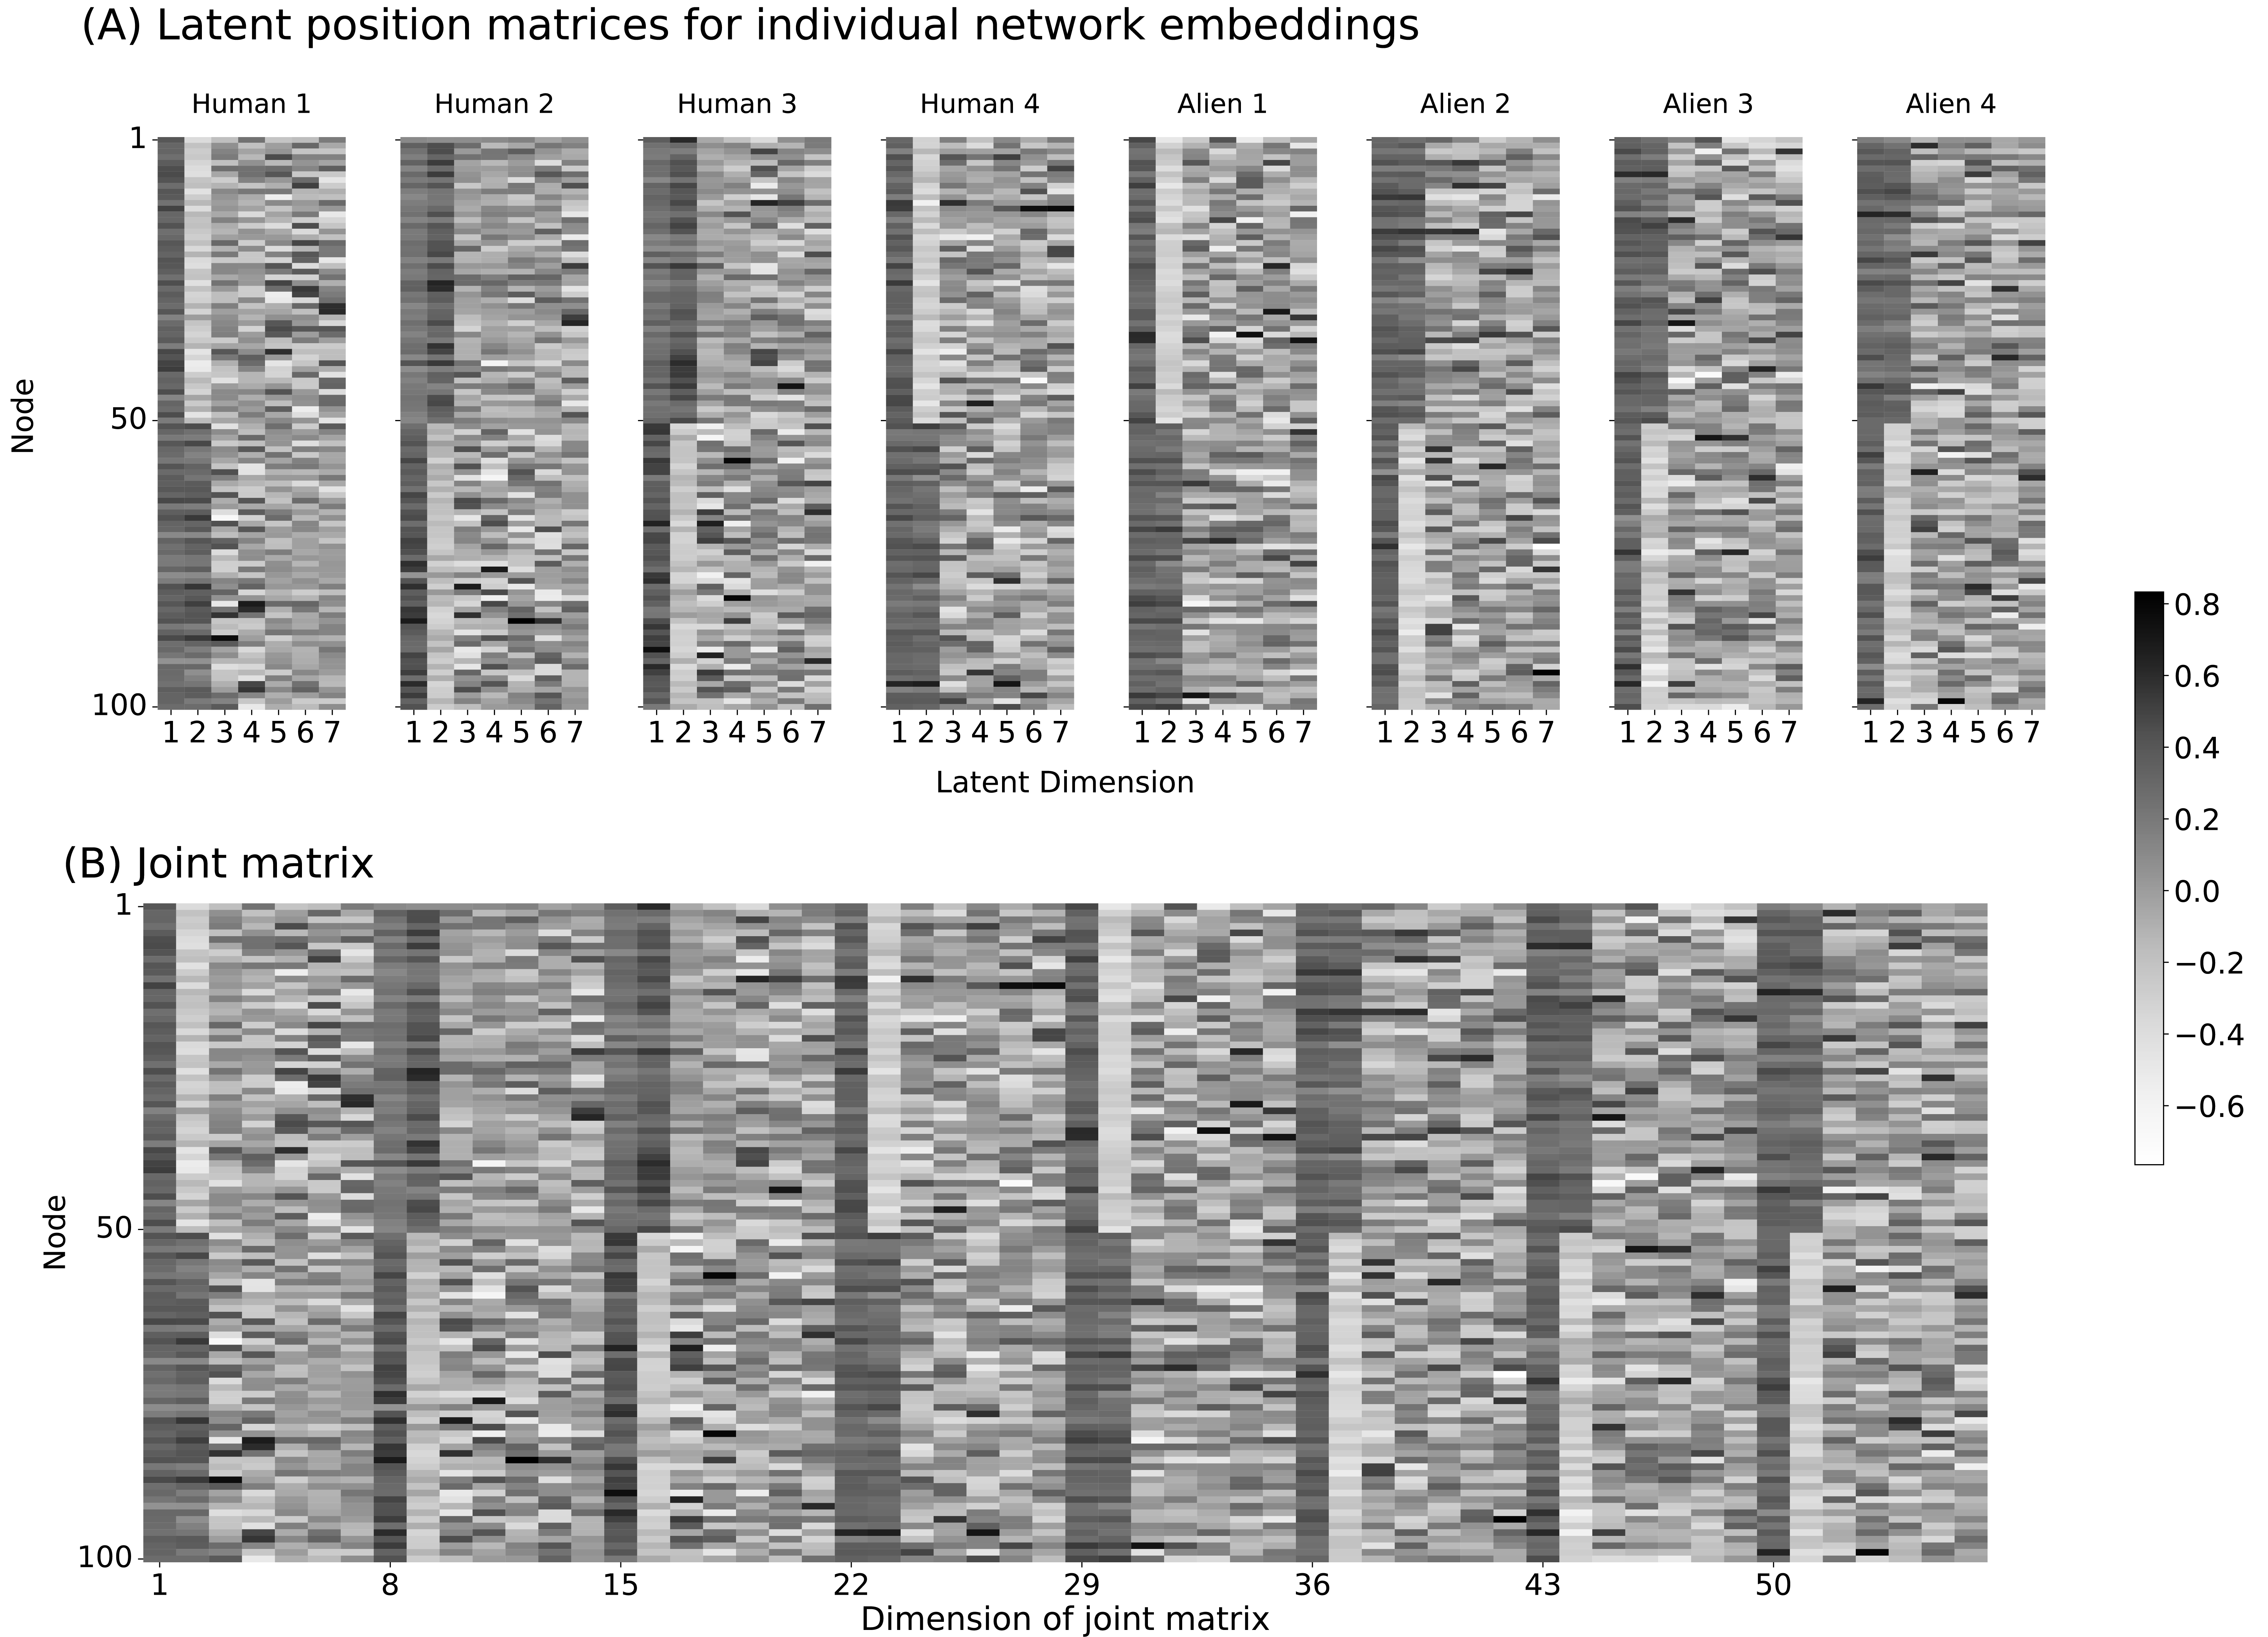
\includegraphics[width=\linewidth]{representations/ch6/Images/mase_embed_joint.png}
    \caption[\texttt{mase} joint matrix]{\textbf{(A)} the separate embeddings for each network. \textbf{(B)} the joint matrix, which concatenates the separate embeddings for each network (horizontally).}
    \label{fig:ch6:multinet:mase:ase_joint}
\end{figure}

When we look at the joint matrix oriented in this manner, we can see the property that we are going to exploit in our next step. Notice that there looks to be a lot of redundant information in this matrix. In particular, the first column always appears to be relatively constant across all of the networks. The second column of every embedding looks like it tends to separate the first $50$ nodes (which were the left hemisphere) from the next $50$ nodes (which were the right hemisphere). Successive dimensions tend to look like noise.

This sort of redundancy of some of the qualitative features of the columns is, in fact, exploitable. This is despite the fact that the columns aren't exactly identical in their behavior (for instance, for some of the networks, the second embedding dimension has high values for the first 50 nodes and low values for the second 50 nodes, or low values for the first 50 nodes and high values for the second 50 nodes). The important idea is that there is some notion of similar information being conveyed that we can use to simplify this problem even further.

\paragraph{Embedding the joint matrix to create a joint embedding}

So now we have a joint matrix, but you have a new issue to address: there's a lot of redundant information which is common to many of these embeddings (such as the second dimension tending to separate the left from the right), and some information common only to a subset of these embeddings (such as that some of the networks have the second dimension having high values for the first group of nodes and low values for the second group of nodes, and vice versa for the other networks). The way in which this redundancy is conveyed is not consistent from embedding to embedding, nor even within network groupings (the patterns in some of the human and alien network embeddings are different, even though the underlying $SBM_n(\vec z, B)$ random networks are homogeneous for networks in the same group), which is an instance of the rotational non-identifiability from Section \ref{sec:ch6:spectral:nonidentifiable} problem.

Fortunately, spectral embedding is an ideal candidate for picking out these sorts of ``redundancies'' that arise across columns of our matrix. Spectral embedding allows us to capture the redundancy of the qualitative aspects of these columns, and obtain the general idea of what they each convey numerically. For this, we will use \texttt{pca}, or Principle Components Analysis. The process is nearly identical to what we did before for \texttt{ase} in Algorithm \ref{alg:ch6:ase}, in that we perform an \texttt{svd}, and retain the top $d$ left singular vectors. This is called an \textit{unscaled spectral embedding}, because we are not weighting the left singular vectors by the square roots of the singular values (like we did in \texttt{ase}).

Through this process, what you are effectively doing is now embedding your joint matrix, to obtain a joint embedding. Let's see how this works. Since the networks have two communities, we'll use $2$ embedding dimensions:

\begin{lstlisting}[style=python]
def unscaled_embed(X, d):
    U, s, Vt = np.linalg.svd(X)
    return U[:,0:d]

Vhat = unscaled_embed(joint_mtx, 2)
\end{lstlisting}

The result of this unscaled embedding is known as an \textit{estimate of the shared latent positions}, and is denoted by the matrix $\hat V$. $\hat V$ has $n$ rows and $d$ columns, so each row $\hat{\vec v}_i$ is an estimate of the shared latent position of node $i$. 

We plot the estimate of the shared latent positions $\hat V$ in Figure \ref{fig:ch6:multinet:mase:shared_lpm}. Note that the estimated shared latent positions convey the shared structure between human and alien brains: the left and right hemispheres are appreciably different. 

\begin{figure}[h]
    \centering
    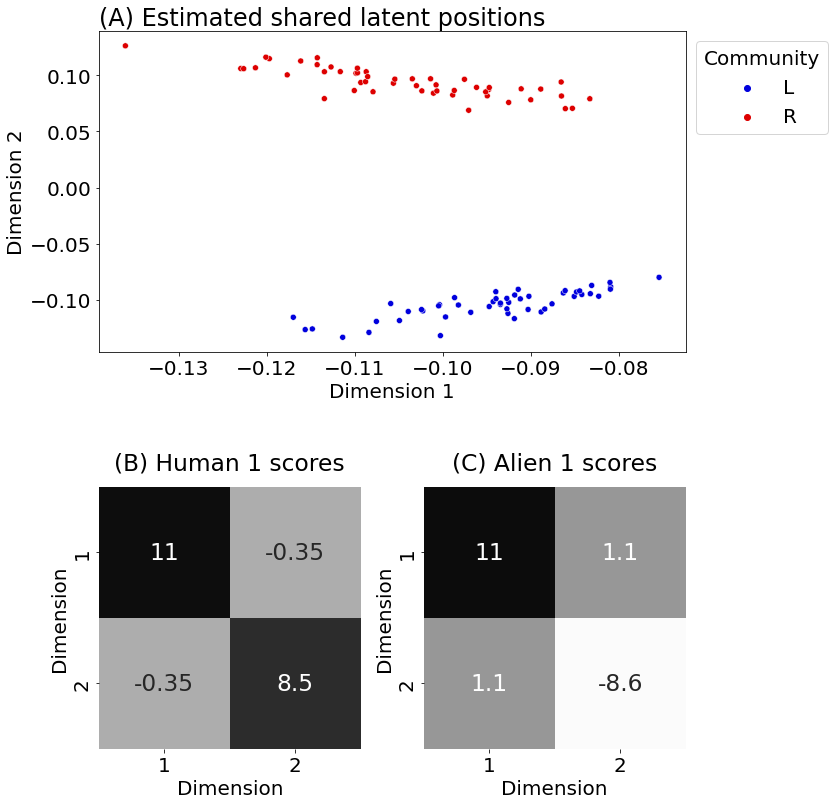
\includegraphics[width=\linewidth]{representations/ch6/Images/mase_shared_lpm.png}
    \caption[parameter estimates from \texttt{mase}]{\textbf{(A)} The estimated shared latent positions of the human and alien brains. \textbf{(B)} the estimated scores for the first human network, \textbf{(C)} the estimated scores for the first alien network.}
    \label{fig:ch6:multinet:mase:shared_lpm}
\end{figure}

\subsubsection{Building representations for each network}

Exactly how is the joint embedding we created related to all of our separate, original networks? Remember that under the COSIE model in Section \ref{sec:ch5:multi:cosie}, the probability matrix for the $i^{th}$ network could be described as:

\begin{align*}
    P^{(i)} &= VR^{(i)}V^\top \numberthis \label{eqn:ch6:mase:e1}
\end{align*}

where $V$ conveyed the homogeneity across all $M$ networks (the \textit{shared latent positions}), and $R^{(i)}$ conveyed the unique aspects of the probability matrix for a particular network $i$ (the unique \textit{score matrices}).

Next, remember that in the COSIE model, an assumption was that $V$ was orthonormal. For an orthonormal matrix $V$ with $n$ rows and $n$ columns, $V^\top V = VV^\top = I_n$. This means that conceptually that by pre-multiplying by $V^\top$ and post-multiplying by $V$ in Equation \eqref{eqn:ch6:mase:e1}:
\begin{align*}
    V^\top P^{(i)}V &= V^\top VR^{(i)} V^\top V \\
    \Rightarrow R^{(i)}&= V^\top P^{(i)} V,\numberthis \label{eqn:ch6:mase:score_est}
\end{align*}
which is because $V$ was orthonormal.

In practice, however, we have two problems.

\paragraph*{Estimates of the shared latent positions are not orthonormal}

We do not have the shared latent positions, we have an estimate of the shared latent positions $\hat V$. $\hat V$ is the first $d$ columns of the left singular vectors $U$ of the joint matrix. While the full left singular vector matrix is orthonormal (by definition of the \texttt{svd}, in Remark \ref{box:ch6:svd_results}), it is generally favorable to \textit{reduce} the dimensionality when we embed, below the number of nodes in the network so that we can learn from the shared latent position matrix later. Unfortunately, this disrupts the orthonormality, and $\hat V$ is no longer orthonormal when we discard the last $n - d$ columns.

\paragraph*{We do not observe the probability matrix}

Remember that a hurdle that we experienced in the \texttt{ase} was that we could obtain a perfect estimate of the latent position matrix (up to a rotation) if we knew the probability matrix. However, we do not have a probability matrix, because the probability matrix was a merely an intuitive construct that we use to conceptualize our network sample, and to evaluate the techniques that we developed if our conceptual model is correct. 

In its place, we simply used the adjacency matrix. The reason that we settled on the approach that we settled on for \texttt{ase} was that the eigendecomposition procedure in Algorithm \ref{alg:ch6:evd} would not work unless the matrix was positive semi-definite, but we had no such restriction with the \texttt{ase} procedure in Algorithm \ref{alg:ch6:ase} that used the \texttt{svd}. Likewise, no part of our procedure for \texttt{mase} is restrictive of positive semi-definiteness to obtain a real answer.

\paragraph*{Ignorance proves blissful (again)}

While these limitations might feel impactful, just like with the \texttt{ase}, we can ignore them (for the time being). Using Equation \eqref{eqn:ch6:mase:score_est} for the score matrices, we simply plug in the estimate of the shared latent positions for $V$, and the adjacency matrix $A^{(i)}$ for the probability matrix, to obtain an estimate of the score matrix:

\begin{align*}
    \hat R^{(i)} &= \hat V^\top A^{(i)}\hat V.
\end{align*}

Let's see how to do this in practice with our networks:

\begin{lstlisting}[style=python]
# stack the networks into a numpy array
As_ar = np.asarray(As)
# compute the scores
scores = Vhat.T @ As_ar @ Vhat
\end{lstlisting}
We plot the estimated score matrices in Figure \ref{fig:ch6:multinet:mase:shared_lpm}(B) and (C) for a human and alien network, respectively. Notice in particular that the human networks and the alien networks leverage different combinations of the two latent dimensions to ``reconstruct'' the score matrix, much like in Section \ref{sec:ch5:multi:cosie:score} when the Facebook/Twitter and Linkedin networks used different score matrices to convey the disparate structure in the networks. In particular, the second estimated shared latent dimension, which is the shared latent dimension that conveys the disparity between the left and right communities, is much different for the human and alien networks. This highlights that the human and alien networks convey the disparate community structure (humans having a homophilic structure, aliens a dissassortative structure) through the latent dimension which distinguishes the communities.

Finally, we use this with the COSIE model in Equation \eqref{eqn:ch6:mase:e1} to obtain that:
\begin{align*}
    \hat P^{(i)} &= \hat V \hat R^{(i)} \hat V^\top.
\end{align*}
Let's see how this works out in practice, by computing the true probability matrix for the humans and aliens, and comparing it to the estimated probability matrix for the humans and aliens. We compute the true probability matrix using the results from Section \ref{sec:ch5:ier:sbm_pmtx}.

\begin{lstlisting}[style=python]
from graphbook_code import generate_sbm_pmtx

Phum = generate_sbm_pmtx(zs, Bhum)
Palien = generate_sbm_pmtx(zs, Balien)
Pests = Vhat @ scores @ Vhat.T
\end{lstlisting}

The true probability matrices for humans and aliens are shown in Figure \ref{fig:ch6:multinet:mase:est_prob}(A) and (C), and are compared to the estimated probability matrices for aliens and humans are shown in Figure \ref{fig:ch6:multinet:mase:est_prob}(B) and (D). Note that \texttt{mase} is able to recover both the homophilic structure of the human brain networks and the disassoratative structure of the alien brain networks across estimated shared latent dimension 2 in Figure \ref{fig:ch6:multinet:mase:shared_lpm}(A), which separated the left and right communities. 

\begin{figure}[h]
    \centering
    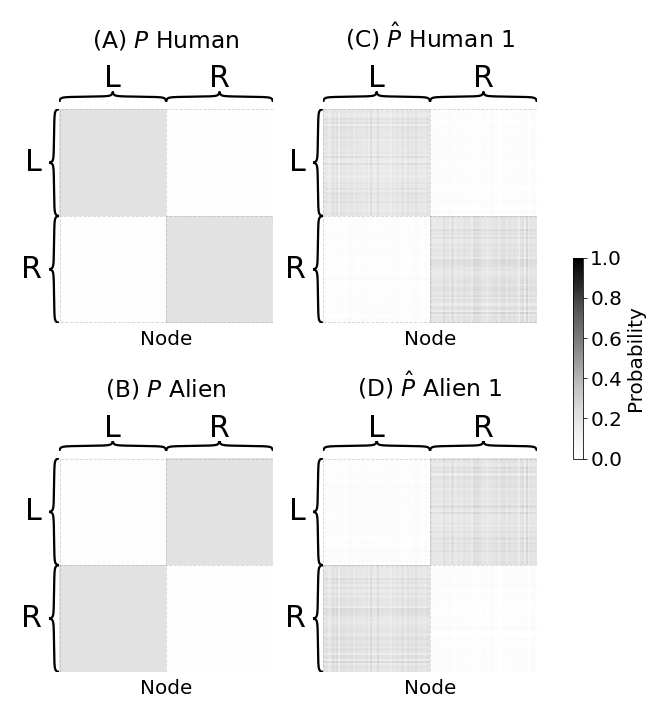
\includegraphics[width=0.8\linewidth]{representations/ch6/Images/mase_probs.png}
    \caption[probability matrix estimates for \texttt{mase}]{\textbf{(A)} the probability matrix for human networks, \textbf{(B)} the estimated probability matrix for the first human network. \textbf{(C)} the probability matrix for alien networks, \textbf{(D)} the estimated probability matrix for the first alien network.}
    \label{fig:ch6:multinet:mase:est_prob}
\end{figure}

\subsubsection{Using \texttt{mase} in practice}

The \texttt{mase} algorithm is shown in Algorithm \ref{alg:ch6:mase}. 

\begin{algorithm}[h]\caption{Multiple adjacency spectral embedding (\texttt{mase})}
\label{alg:ch6:mase}
\KwData{$A^{(1)}, ..., A^{(M)}$ a collection of $M$ networks with $n$ nodes.\newline $d$ the desired latent dimensionality.}
\KwResult{the estimated shared latent position matrix and the estimated score matrices.}
\SetAlgoLined

For each $A^{(i)}$, obtain $\hat X^{(i)} = \texttt{ase}\left(A^{(i)}, \log_2(n)\right)$, for $i = 1, \hdots, M$, via Algorithm \ref{alg:ch6:ase}. 

Let $J = \begin{bmatrix}\hat X^{(1)} & \hdots & \hat X^{(M)}\end{bmatrix}$ be the joint matrix, consisting of a column-wise concatenation of the individual estimated latent position matrices.

Let $U, \Sigma, V = \texttt{svd}(J)$.

Let $\hat V = U_d$, the first $d$ columns of the left singular vectors of $J$. 

Let $\hat R^{(i)} = \hat V^\top A^{(i)}\hat V$, for $i = 1, \hdots, M$.

\Return{$\hat V, R^{(1)}, \hdots, R^{(M)}$}
\end{algorithm}

You can run the \texttt{mase} algorithm using \texttt{graspologic}, which streamlines the procedure that we outlined above:

\begin{lstlisting}[style=python]
from graspologic.embed import MultipleASE as mase

d = 2
mase_embedder = mase(n_components=d)
# obtain an estimate of the shared latent positions
Vhat = mase_embedder.fit_transform(As)
# obtain an estimate of the scores
Rhat_hum1 = mase_embedder.scores_[0]
# obtain an estimate of the probability matrix for the first human
Phat_hum1 = Vhat @ mase_embedder.scores_[0] @ Vhat.T
\end{lstlisting}

\subsection{Omnibus Embedding}
\label{sec:ch6:multinet:omni}

The \textit{Omnibus Embedding} (\texttt{omni}) embeds networks separately while keeping them all into the same latent space (that is, they will be properly rotated to align with one another). What this means is that the embeddings for each network after the omnibus embedding can be compared. \texttt{omni} does not attempt to separately identify shared and unique structures across networks, unlike \texttt{mase} (which considered shared structures via the estimated shared latent positions and unique structure through the separate estimated score matrices for each network).

\subsubsection{How does \texttt{omni} work?}

\paragraph*{Computing the omnibus matrix}

The first step in \texttt{omni} is to compute the omnibus matrix, which is the joint matrix used by \texttt{omni}. The \textit{omnibus matrix} for a collection of $M$ networks with $n$ nodes is the $Mn \times Mn$ matrix $O$, where for each $n \times n$ block $O^{(i, j)}$, it is:
\begin{align*}
    O^{(i, j)} &= \frac{1}{2}\left(A^{(i)} + A^{(j)}\right).
\end{align*}
The resulting $(i, j)$ block of the omnibus matrix is itself a $n \times n$ matrix, and the Omnibus matrix looks like this:
\begin{align*}
    O &= \begin{bmatrix}
        O^{(1, 1)} & \hdots & O^{(1, M)} \\
        \vdots & \ddots & \vdots \\
        O^{(M, 1)} & \hdots & O^{(M, M)}
    \end{bmatrix} = \begin{bmatrix}
        A^{(1, 1)} & \hdots & \frac{1}{2}\left(A^{(1)} + A^{(M)}\right) \\
        \vdots & \ddots & \vdots \\
        \frac{1}{2}\left(A^{(1)} + A^{(M)}\right) & \hdots &  A^{(M)}
    \end{bmatrix}.
\end{align*}
By construction, notice that the Omnibus matrix is symmetric with respect to the blocks themselves, in that $O^{(i, j)} = O^{(j, i)}$. However, if these individual blocks are not themselves symmetric, the omnibus matrix might not be symmetric. Since the blocks of the omnibus matrix are combinations of adjacency matrices, and adjacency matrices are symmetric when the underlying networks are undirected, the omnibus matrix is symmetric when the collection of networks are undirected. 

Let's consider only the first two networks (human networks), and construct a simple omnibus matrix from these. We can do this with \texttt{numpy}:

\begin{lstlisting}[style=python]
omni_ex = np.block([[As[0], (As[0]+As[1])/2],
                 [(As[1]+As[0])/2, As[1]]])
\end{lstlisting}

We visualize this small omnibus matrix in Figure \ref{fig:ch6:multinet:omni:ex}. We illustrate the first two networks in \ref{fig:ch6:multinet:omni:ex}(A) and \ref{fig:ch6:multinet:omni:ex}(B), and the resulting omnibus matrix of the first two networks in \ref{fig:ch6:multinet:omni:ex}(C).

\begin{figure}[h]
    \centering
    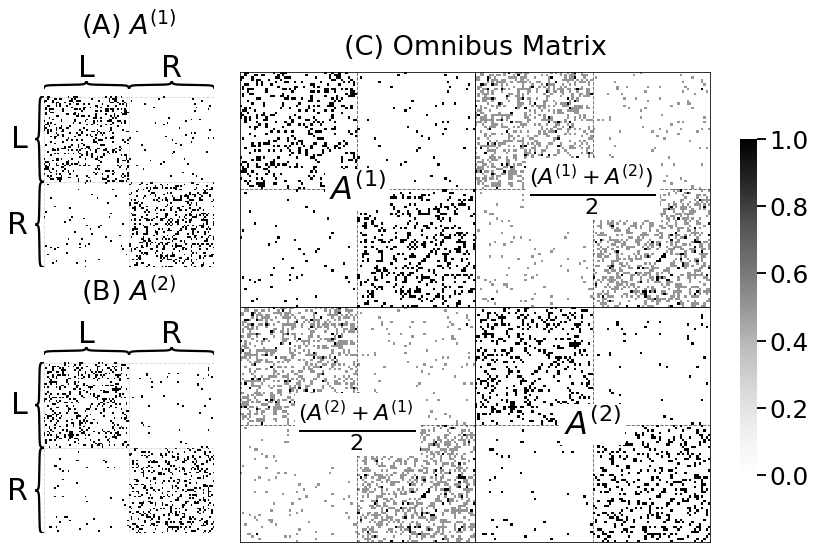
\includegraphics[width=\linewidth]{representations/ch6/Images/omni_ex.png}
    \caption[simple example of omnibus matrix]{\textbf{(A)} the first human network, \textbf{(B)} the second human network. \textbf{(C)} the omnibus matrix of the first two human networks.}
    \label{fig:ch6:multinet:omni:ex}
\end{figure}

We can use \texttt{graspologic} to obtain the omnibus matrix for our collection of networks:
\begin{lstlisting}[style=python]
from graspologic.embed.omni import _get_omni_matrix
omni_mtx = _get_omni_matrix(As)
\end{lstlisting}

The full omnibus matrix for all $8$ networks is shown in Figure \ref{fig:ch6:multinet:omni:fullmtx}(A). You can conceptualize the omnibus matrix as the adjacency matrix of a new network from your collection of networks, where the nodes from each network form a single node in the new network. A subnetwork induced on the omnibus matrix by the nodes from a single network is the original network itself (the on-diagonal blocks of the omnibus matrix $O^{(i,i)}$). The subnetwork formed by the nodes of a network $i$ and the nodes of another network $j$ provides information about how similar (or different) the networks $i$ and $j$ are (the off-diagonal blocks of the omnibus matrix $O^{(i, j)}$). This incorporation of information about each network in relation to the other networks is what will allow \texttt{omni} to properly orient the latent positions across your collection of networks.

\paragraph*{Embedding the omnibus matrix}

The next step to \texttt{omni} is to embed the omnibus matrix using \texttt{ase}. This creates an estimate of the latent position matrix for the omnibus matrix itself. When you embed the $Mn \times Mn$ omnibus matrix into $d$ dimensions, you obtain an estimated latent position matrix that has $Mn \times d$ dimensions. A good rule of thumb for the omnibus embedding is to use $\log_2(n)$ embedding dimensions.

\begin{figure}[h]
    \centering
    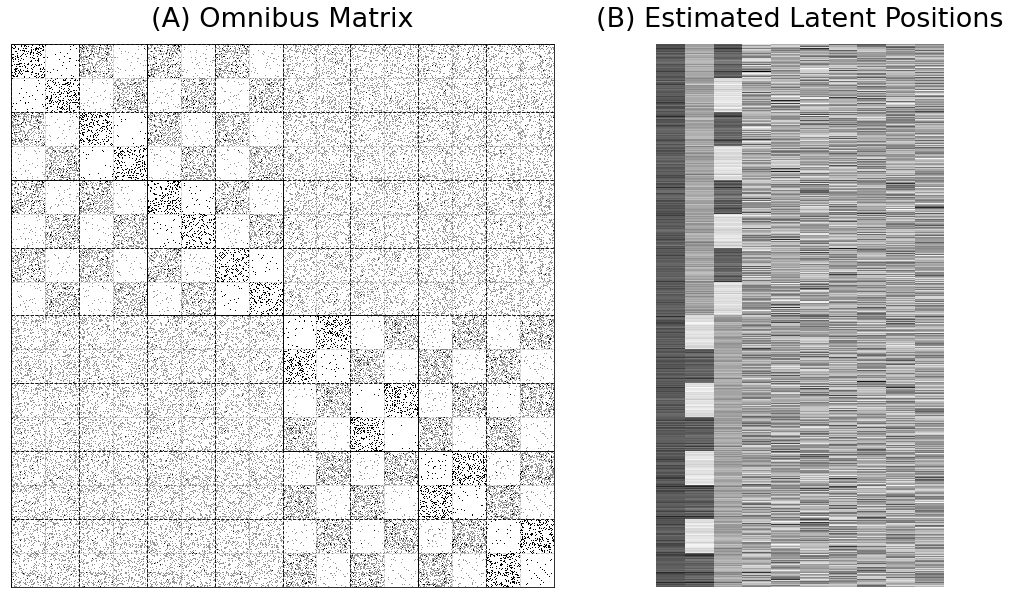
\includegraphics[width=\linewidth]{representations/ch6/Images/omni_mtx.png}
    \caption[omnibus matrix and omnibus embedding]{\textbf{(A)} the omnibus matrix, and \textbf{(B)} the embedded omnibus matrix.}
    \label{fig:ch6:multinet:omni:fullmtx}
\end{figure}

\begin{lstlisting}[style=python]
from graspologic.embed import AdjacencySpectralEmbed as ase

dhat = int(np.ceil(np.log2(n)))
Xhat_omni = ase(n_components=dhat).fit_transform(omni_mtx)
\end{lstlisting}

The estimated latent positions for the omnibus matrix are shown in Figure \ref{fig:ch6:multinet:omni:fullmtx}.

\paragraph*{Extracting oriented estimated latent positions}

The last step of \texttt{omni} is to obtain the properly oriented latent position estimates for each network. Remember that the omnibus matrix effectively could be conceptualized as the adjacency matrix for a new network, where the $Mn$ nodes of this new network are the $n$ nodes of each of the original $M$ networks. Visually, the $Mn \times d$ estimated latent position matrix looks like this:
\begin{align*}
    \hat X &= \begin{bmatrix}
        \hat X^{(1)} \\
        \hat X^{(2)} \\
        \vdots \\
        \hat X^{(M)}
    \end{bmatrix},
\end{align*}
where each set of estimated latent positions $\hat X^{(i)}$ which are $n \times d$ matrices correspond to the estimated latent positions for the network $A^{(i)}$.

To obtain the latent positions for each network explicitly, you can reshape the $Mn \times d$ matrix into an $m \times n \times d$ tensor, and look at the individual slices of the tensor corresponding to the estimated latent position matrix for each network. You can do this with \texttt{numpy} like this:

\begin{lstlisting}[style=python]
M = len(networks)
n = len(networks[0])

# obtain a M x n x d tensor
Xhat_tensor = Xhat_omni.reshape(M, n, -1)
# the estimated latent positions for the first network
Xhat_hum1 = Xhat_tensor[0,:,:]
\end{lstlisting}

The estimated latent positions for each network are illustrated in Figure \ref{fig:ch6:multinet:omni:individual} for all of the networks in our collection. The second and third dimensions capture most of the signal disparity between the human and alien networks, so we show scatter plots for these two dimensions. Note that the human networks appear to have the nodes in the same relative positions, and the alien networks appear to have the nodes in the same relative positions, which is a function of the rotational alignment created by \texttt{omni}. Had we embedded the networks separately, this would not have been the case. On the other hand, note that the human brain network nodes and the alien brain network nodes appear to have different patterns in the embeddings, which is a function of the unique disparities between human and alien brain networks.

\begin{figure}[h]
    \centering
    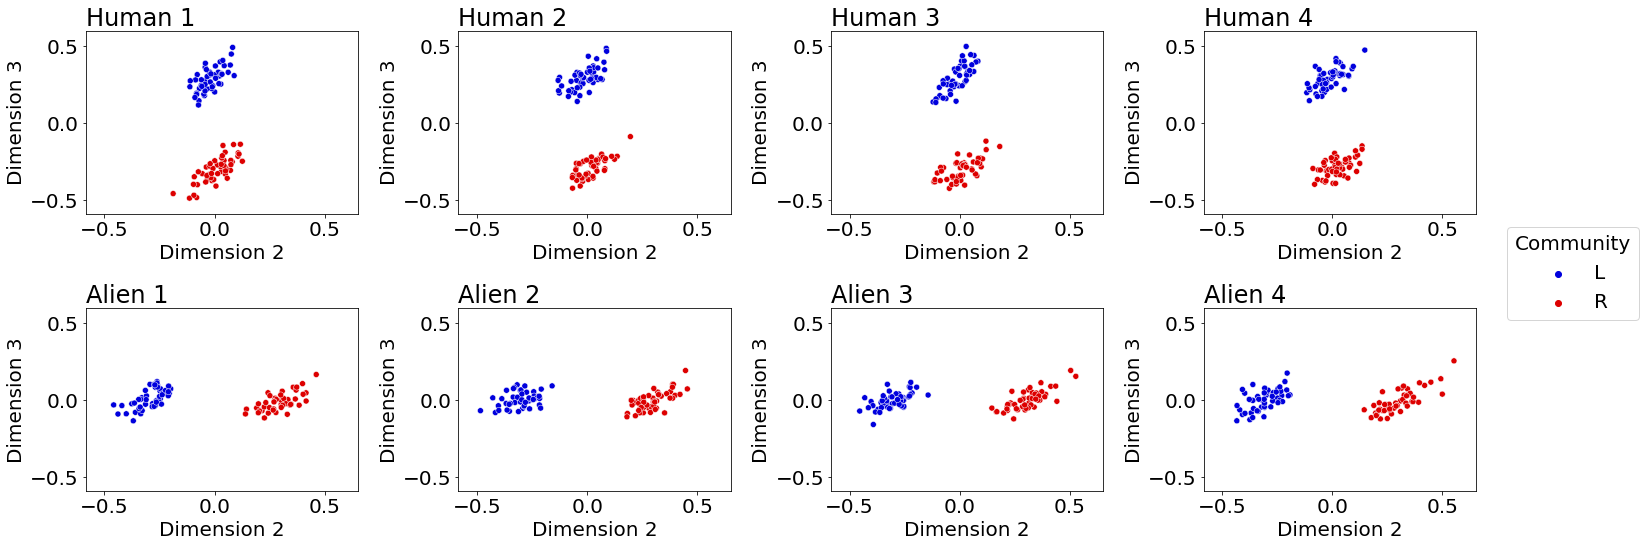
\includegraphics[width=\linewidth]{representations/ch6/Images/omni_ind.png}
    \caption[OMNI estimated latent positions]{The estimated latent positions for each network.}
    \label{fig:ch6:multinet:omni:individual}
\end{figure}

\paragraph*{Using \texttt{omni} in practice}

The procedure for the \texttt{omni} embedding is outlined in Algorithm \ref{alg:ch6:omni}. 



\begin{algorithm}[h]\caption{Omnibus Embedding (\texttt{omni})}
\label{alg:ch6:omni}
\KwData{$A^{(1)}, ..., A^{(M)}$ a collection of $M$ networks with $n$ nodes.\newline $d$ the desired latent dimensionality.}
\KwResult{estimated latent positions for each network.}
\SetAlgoLined

Compute the $Mn \times Mn$ omnibus matrix $O$, where each $n \times n$ submatrix $O^{(i,j)} = \frac{1}{2}\left(A^{(i)} + A^{(j)}\right)$.

Embed the omnibus matrix to produce estimated latent positions for the omnibus network, $\hat X = \texttt{ase}(O, d)$, according to Algorithm \ref{alg:ch6:ase}. 

Let $\hat X^{(i)}$ be the $n \times d$ matrix consisting of the $(i - 1)\cdot n + 1$ through $i\cdot n$ rows of $\hat X$.

\Return{$\hat X^{(1)}, \hdots, \hat X^{(M)}$}
\end{algorithm}

You can run \texttt{omni} using \texttt{graspologic}, as:

\begin{lstlisting}[style=python]
from graspologic.embed import OmnibusEmbed as omni

# obtain a tensor of the estimated latent positions
Xhat_tensor = omni(n_components=int(np.log2(n))).fit_transform(As)
# obtain the estimated latent positions for the first human
# network
Xhat_hum1 = Xhat[0,:,:]
\end{lstlisting}

\subsubsection{Relating \texttt{omni} to heterogeneous collections of RDPGs}

Recall from Chapter \ref{sec:ch5:multi} that a heterogeneous collection of random networks was a collection $\left\{\mathbf A^{(1)}, \hdots, \mathbf A^{(M)}\right\}$ where the underlying probability matrices $\left\{P^{(1)}, \hdots, P^{(M)}\right\}$ are not all the same. Therefore, for at least two networks $i$ and $j$, $P^{(i)} \neq P^{(j)}$.

If you think that a heterogeneous collection of random networks are each reasonably described by positive semi-definite probability matrices $P^{(i)}$, the underlying network model is that each random network $\mathbf A^{(i)}$ is an $RDPG_n\left(\mathbf X^{(i)}\right)$ random network. 

When we produced an embedding of each network using \texttt{omni}, what we did was we produced estimates $\hat X^{(i)}$ for each of our $M$ networks. 

With this framework in mind, the estimates $\hat X^{(i)}$ are interpretable as estimates of latent position matrices for each network $i$, and we can evaluate the estimated probability matrix $\hat P^{(i)} = \hat X^{(i)} \hat X^{(i)}^\top$. 

Using \texttt{omni}, you can obtain the estimates of probability matrices like this:

\begin{lstlisting}[style=python]
Phat_hum1 = Xhat_hum1 @ Xhat_hum1.T
\end{lstlisting}

Repeating this for both human and alien networks, you should be able to convince yourself that this conceptual model does a reasonable job of estimating the underlying probability matrices for our networks, like we did for \texttt{mase}.

\subsection{When should you use \texttt{omni} versus \texttt{mase}?}

Both \texttt{omni} and \texttt{mase} will produce estimated latent representations of collections of networks that will allow you to compare these estimated latent representations downstream in your analysis. In this sense, these techniques take a collection of networks, and tabularize them in such a way that you can compare the tabularized representations of the networks with tabular machine learning strategies. 

Note that \texttt{mase} effectively summarizes each network individually prior to the construction of the joint matrix, by first taking the \texttt{ase} of each individual network. The joint matrix is an $n \times Md$ matrix, where $d$ is the number of embedding dimensions that you use in the \texttt{ase} sub-step of \texttt{mase} (and is usually taken to be $\log_2(n)$). This matrix is rather manageable in size/scale for successive operations, as the number of elements is scaling on the order of $n\sqrt n$ and $M$.

\texttt{omni} has as substantial limitation: the construction (and embedding) of the omnibus matrix. The omnibus matrix scales in size with $(Mn)^2$, which can get quite computationally expensive very quickly. When you have many networks and $M$ is large, or when you have many nodes per network and $n$ is large, this can be quite computationally prohibitive to analyze. The \texttt{svd} can be quite intensive to compute with sizable matrices, and therefore in practice you might find \texttt{mase} to be simpler to incorporate into your analysis without having to make these computational considerations.

Both \texttt{omni} and \texttt{mase} are fairly simple to use, and have very similar theoretical underpinnings (\texttt{mase} on the COSIE model, and \texttt{omni} on the heterogeneous RDPG model), and are relatively intuitively flexible. While the COSIE model makes explicit use of shared structure, there is nothing prohibiting the COSIE model from incorporating little to no shared structure across your collection of networks (if none is present). We could imagine a situation where in the worst case where there is no shared structure, the estimated ``shared'' latent positions could be taken to be unique latent positions for each network. Then, the score matrices for each network could leverage only the unique latent positions for that specific network (and simply have scores of $0$ for the estimated shared latent positions that are associated with other networks). For this reason, when you want to exploit or highlight shared/unique structures across your collection of networks, \texttt{mase} is a very sensible choice to use.

A nice feature of \texttt{omni} is that it produces latent position estimates for each network, rather than just unique score matrices for each network. This means that for each network, you end up with a $d$-dimensional representation for each node. If you want to learn about disparities across your networks downstream at the node-wise level, this might be a very reasonable starting point for your analysis, and might be more direct to incorporate with tabular machine learning techniques that you are already familiar with.

For these reasons, our advice would be, if computational time or spatial considerations need to be made, or if you anticipate some amount of shared structure in your networks, \texttt{mase} might be more reasonable to use for your analysis. If you do not anticipate shared structure in your networks, either \texttt{mase} or \texttt{omni} are principled approaches to proceeding, and you could identify a strategy on the basis of the representation (estimated shared latent position matrices and unique score matrices, or unique estimated latent positions) that you are most comfortable working with.

\newpage